\section{Evaluation}
To evaluate the performance of our extracted features and proposed feature-based transfer regression models, we conduct a series of experiments to check both the performance of \textit{local transfer} and \textit{cross-region transfer}.
In this section, we first discuss the setup of our experiments, then the baseline methods and finally present the discussion of the experimental results.
\subsection{Experiment Setup}
We first split the data into training set and test set with respect to the time. 
Specifically, we first split the data in 2013 into two parts (Jan. - Jun.) and (Jul. - Dec.).
Three scenarios are shown as follows:
1)~\textit{\textbf{No Transfer}} task is to predict the future speed  (the second half year) of a link with the historical (the first half year) data of the link.		
2)~\textit{\textbf{Local Transfer}} task is to consider the data in first half year as training data and second half year data as test data. 
We train the models for each region with their data and test the models with the testing data in the same region. 
3)~\textit{\textbf{Cross-region Transfer}} task is to use a model trained on the first half year data of a source region to predict the traffic speed of another target region in the second half year.
%For example, trained model on Brooklyn to predict the speed of Queens.

\subsection{Baseline Methods}
To compare our model with the most common time-series based regression model, we choose two representative ones: ARIMA~\cite{ARIMA} and HAM. 
	\subsubsection{Auto-Regressive Integrated Moving Average (ARIMA)}
%	ARIMA model is a generalization of an autoregressive moving average model. 
%	Both of these models are fitted to time series data either to better understand the data or to predict future points in the series (forecasting). 
	ARIMA models are applied on some cases where time series data shows evidence of non-stationarity and an initial differencing step (corresponding to the "integrated" part of the model) can be applied one or more times to eliminate the non-stationarity.
	Prediction of the data for the time $t+1$  is:
	$$ Y_{t+1} = \sum_{i=1}^p \alpha_i Y_{t-i+1}  + \sum_{i=1}^q \beta_i \epsilon_{t-i+1} + \epsilon_{t+1}$$
	where $Y_t$ refers to a time series data. 
	In the autoregressive component of this model, a linear weighted combination of previous data is calculated, where $p$ refers to the order of this model and $\alpha_i$ refers to the weight of $(t-i+1)$-th reading. 
	As for the second part, the sum of weighted noise from the moving average model is calculated, where $\epsilon$ denotes the noise, $q$ refers to its order and $\beta_i$ represents the weight of $(t-i+1)$-th noise.
	In our experiment, we trained ARIMA on the first half year to pick the parameters with best performance using 5-fold cross-validation.
	
	
	
\subsubsection{Historical Average Model (HAM)}
HAM utilizes the average of previous speed data for the same time and same location to forecast the future data. 
HAM is formulated as follows:
$$  v (t_{d,w} +h ) = \frac{1}{|V(d,w)|} \sum _{s\in V(d,w)} \hspace{-8pt} v(s)$$
where $V(d, w)$ refers to the subset of past observations that happened at the same time $d$ on the same weekday $w$. 
Specifically, $d$ captures the daily effects while $w$ captures the weekly effects. 
$7*24$ average regular speed tables for each link are derived from the data of first half year. 
The model is evaluated by comparing using such tables. 
%For example, if the traffic data of a link to be predicted is  at Monday 8:00AM, the ground true value is compared with the 'Monday' row, '8:00AM' column of its particular table.
%\subsection{Our Methods}
%	\subsubsection{Linear Regression Models}
%		
%	\subsubsection{Neural Network Models}
%	\subsubsection{Support Vector Regression Models}
%%	\subsection{}

 


\subsection{Experimental Results}

We first show the performance of HAM and ARIMA models on the \textit{No Transfer} Task with two metrics (RMSE and MAE) in Table~\ref{tbl:notransfer}.
We found that HAM performs substantially better than the ARIMA model with both metrics, 
which is probably due to the time interval in our data is one hour, quite longer than common time interval length for ARIMA model.
\begin{table}[th!]
	\small
	\centering
	\caption{No Transfer Performance of HAM and ARIMA}
	\label{tbl:notransfer}
	\begin{tabular}{|c|c|c|c|c|}
		\hline
		\textbf{}          & \textbf{\begin{tabular}[c]{@{}c@{}}HAM\\ RMSE\end{tabular}} & \textbf{\begin{tabular}[c]{@{}c@{}}HAM\\ MAE\end{tabular}} & \textbf{\begin{tabular}[c]{@{}c@{}}ARIMA\\ RMSE\end{tabular}} & \textbf{\begin{tabular}[c]{@{}c@{}}ARIMA\\ MAE\end{tabular}} \\ \hline
		\textbf{Total}     & 5.1802                                                  & 3.3152                                                & 6.7106                                                   & 4.2806                                                    \\ \hline
		\textbf{Hudson}    & 8.2871                                                 & 6.0331                                                & 11.5791                                                   & 8.8327                                                  \\ \hline
		\textbf{Manhattan} & 4.4532                                                 & 2.7495                                                & 5.2845                                                   & 3.1740                                                  \\ \hline
		\textbf{Brooklyn}  & 5.2661                                                 & 3.4681                                                & 6.8584                                                   & 4.6273                                                  \\ \hline
		\textbf{Bronx}     & 7.6168                                                 & 5.5544                                                 & 11.2118                                                   & 8.5488                                                  \\ \hline
		\textbf{Queens}    & 6.0233                                                 & 4.0720                                                & 8.2514                                                   & 5.7618                                                  \\ \hline
	\end{tabular}
\end{table}


\begin{figure*}[th!]
	\centering
	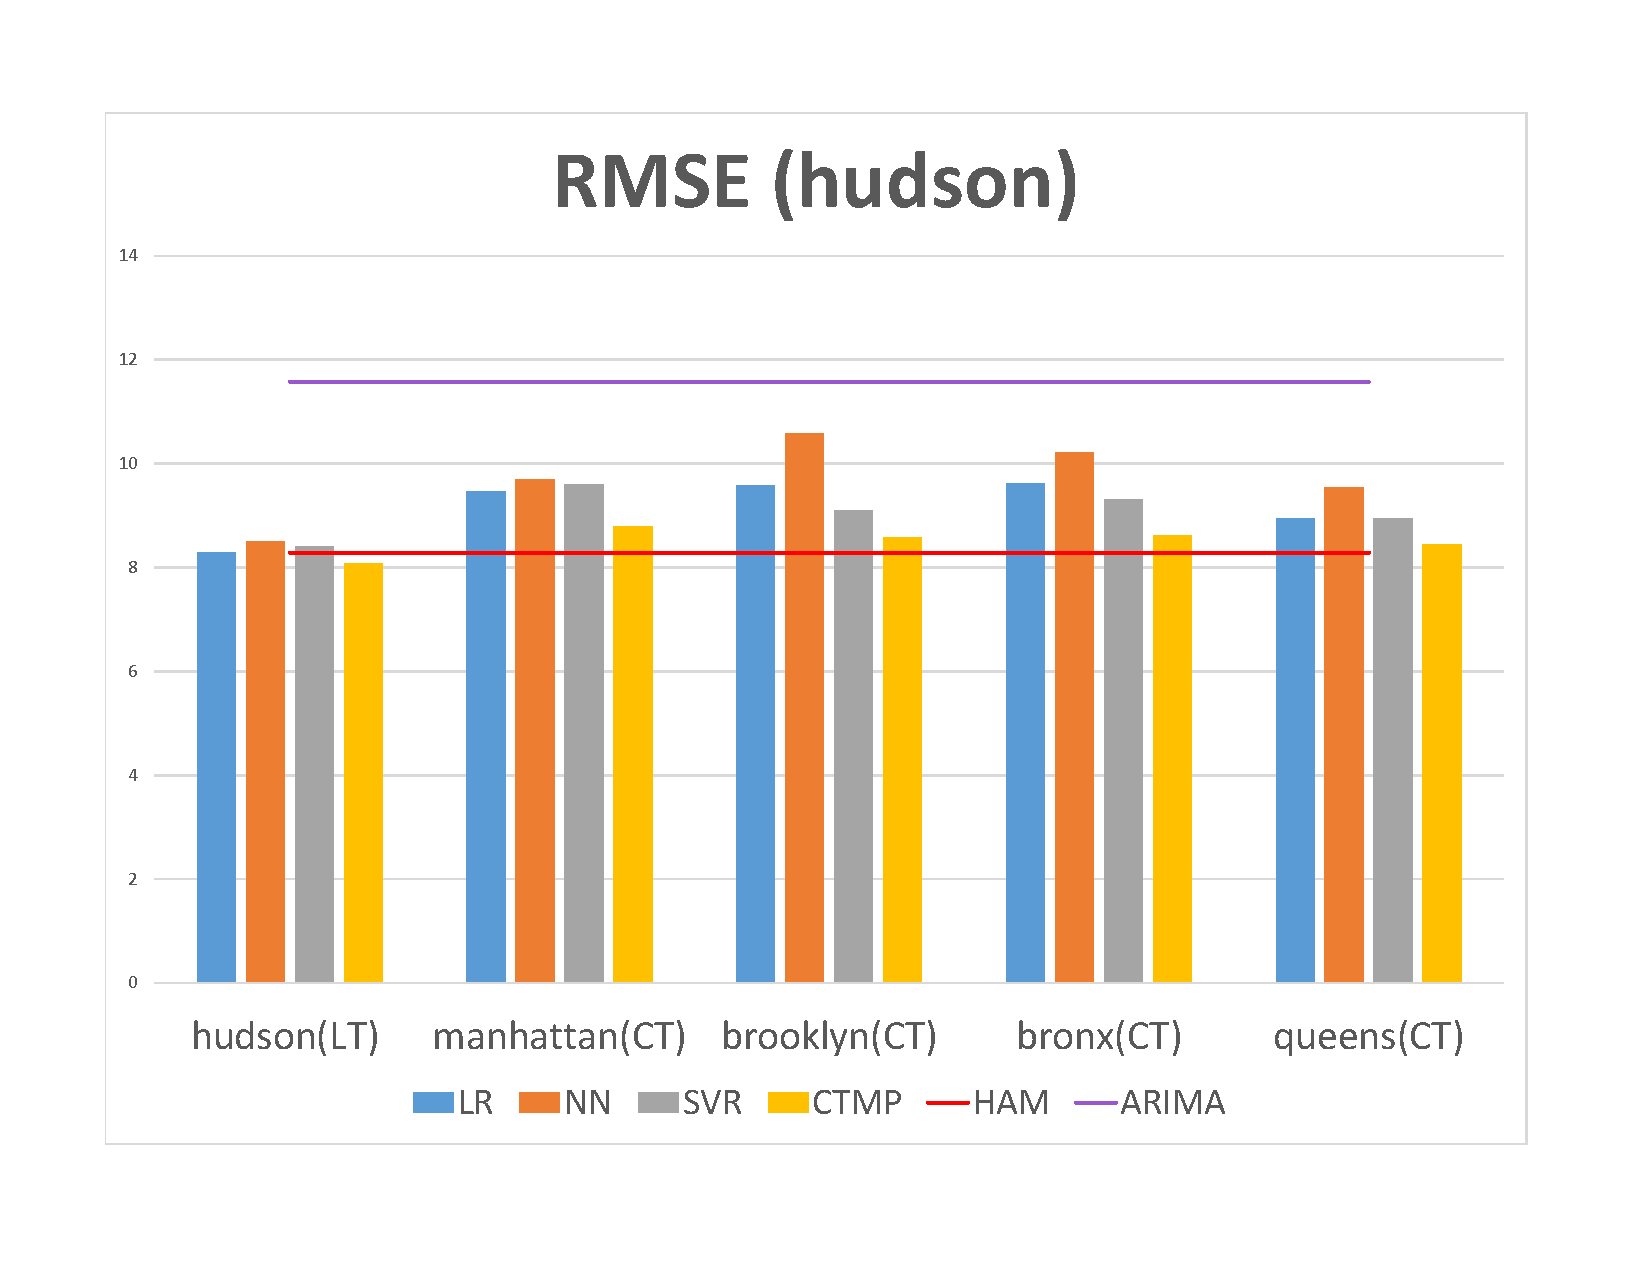
\includegraphics[width=0.34\textwidth]{figures/1.pdf}
	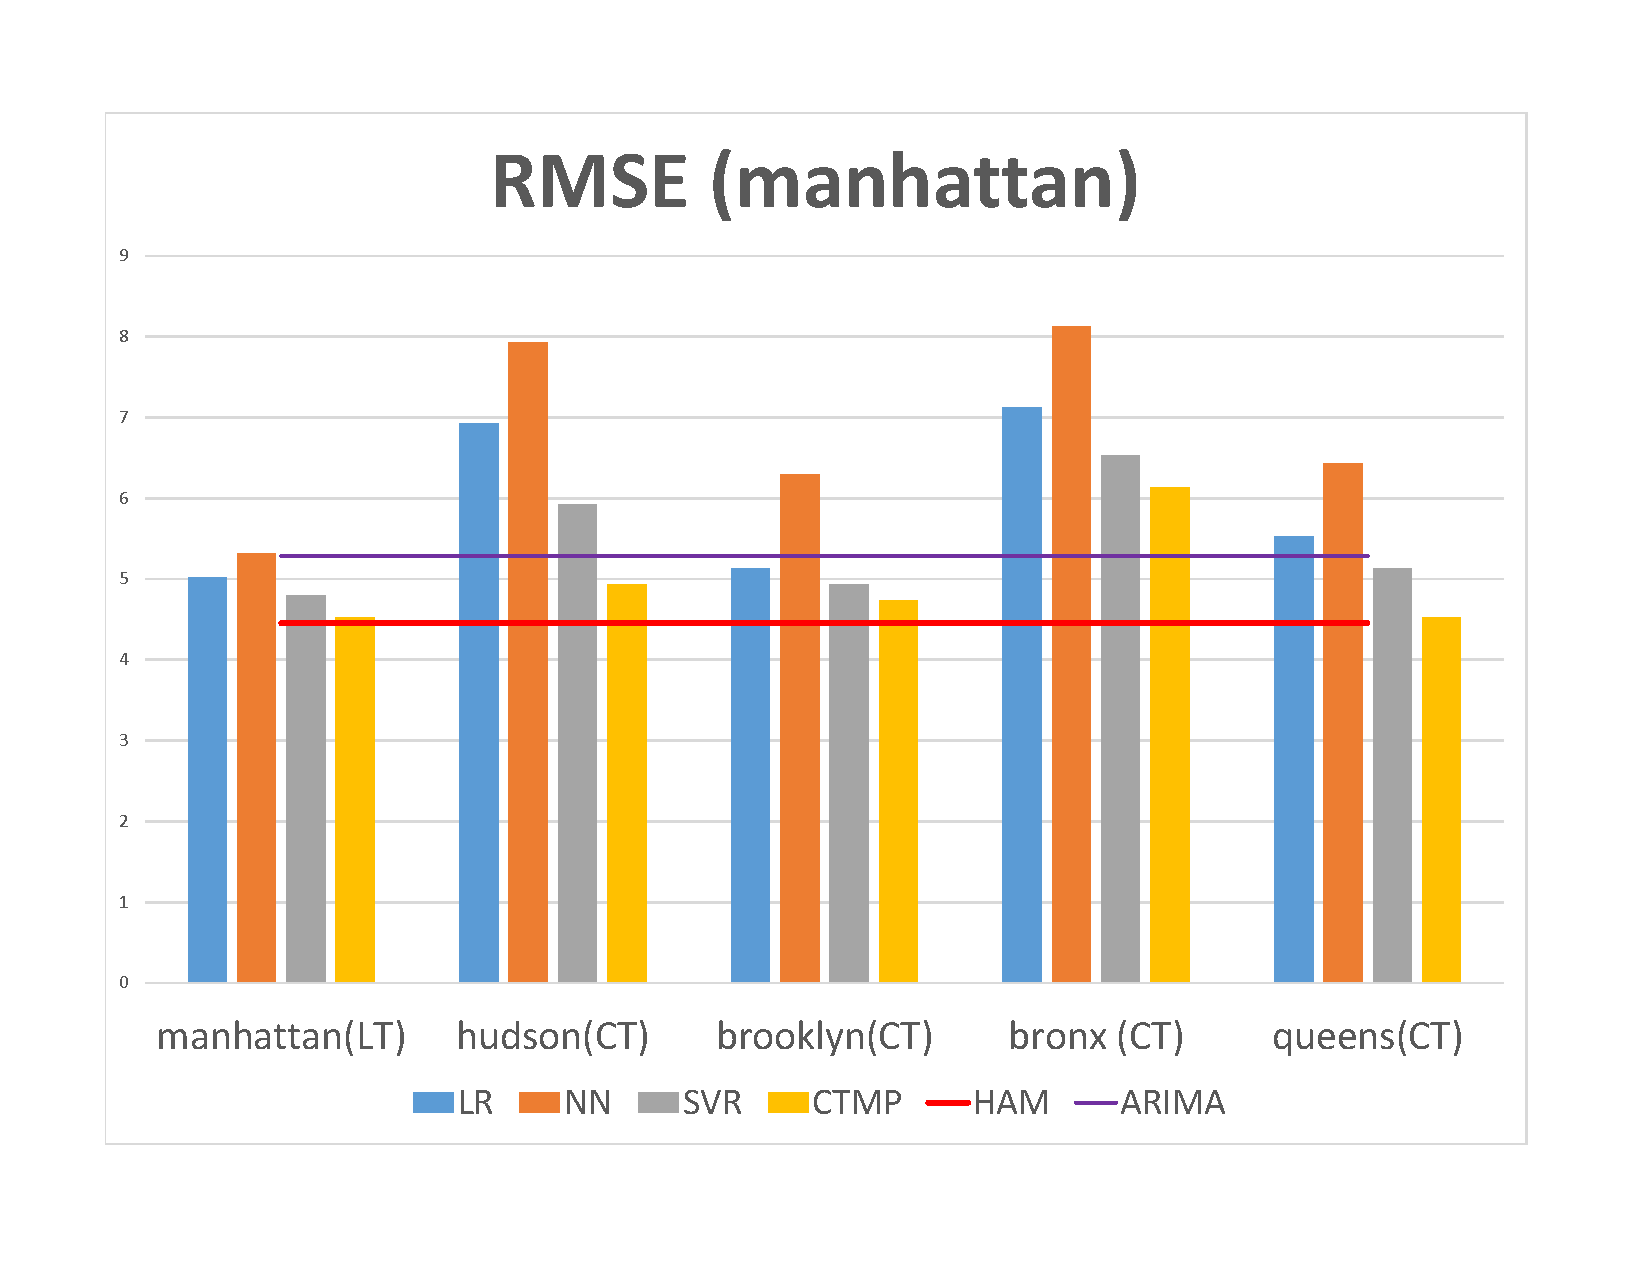
\includegraphics[width=0.34\textwidth]{figures/2.pdf}
	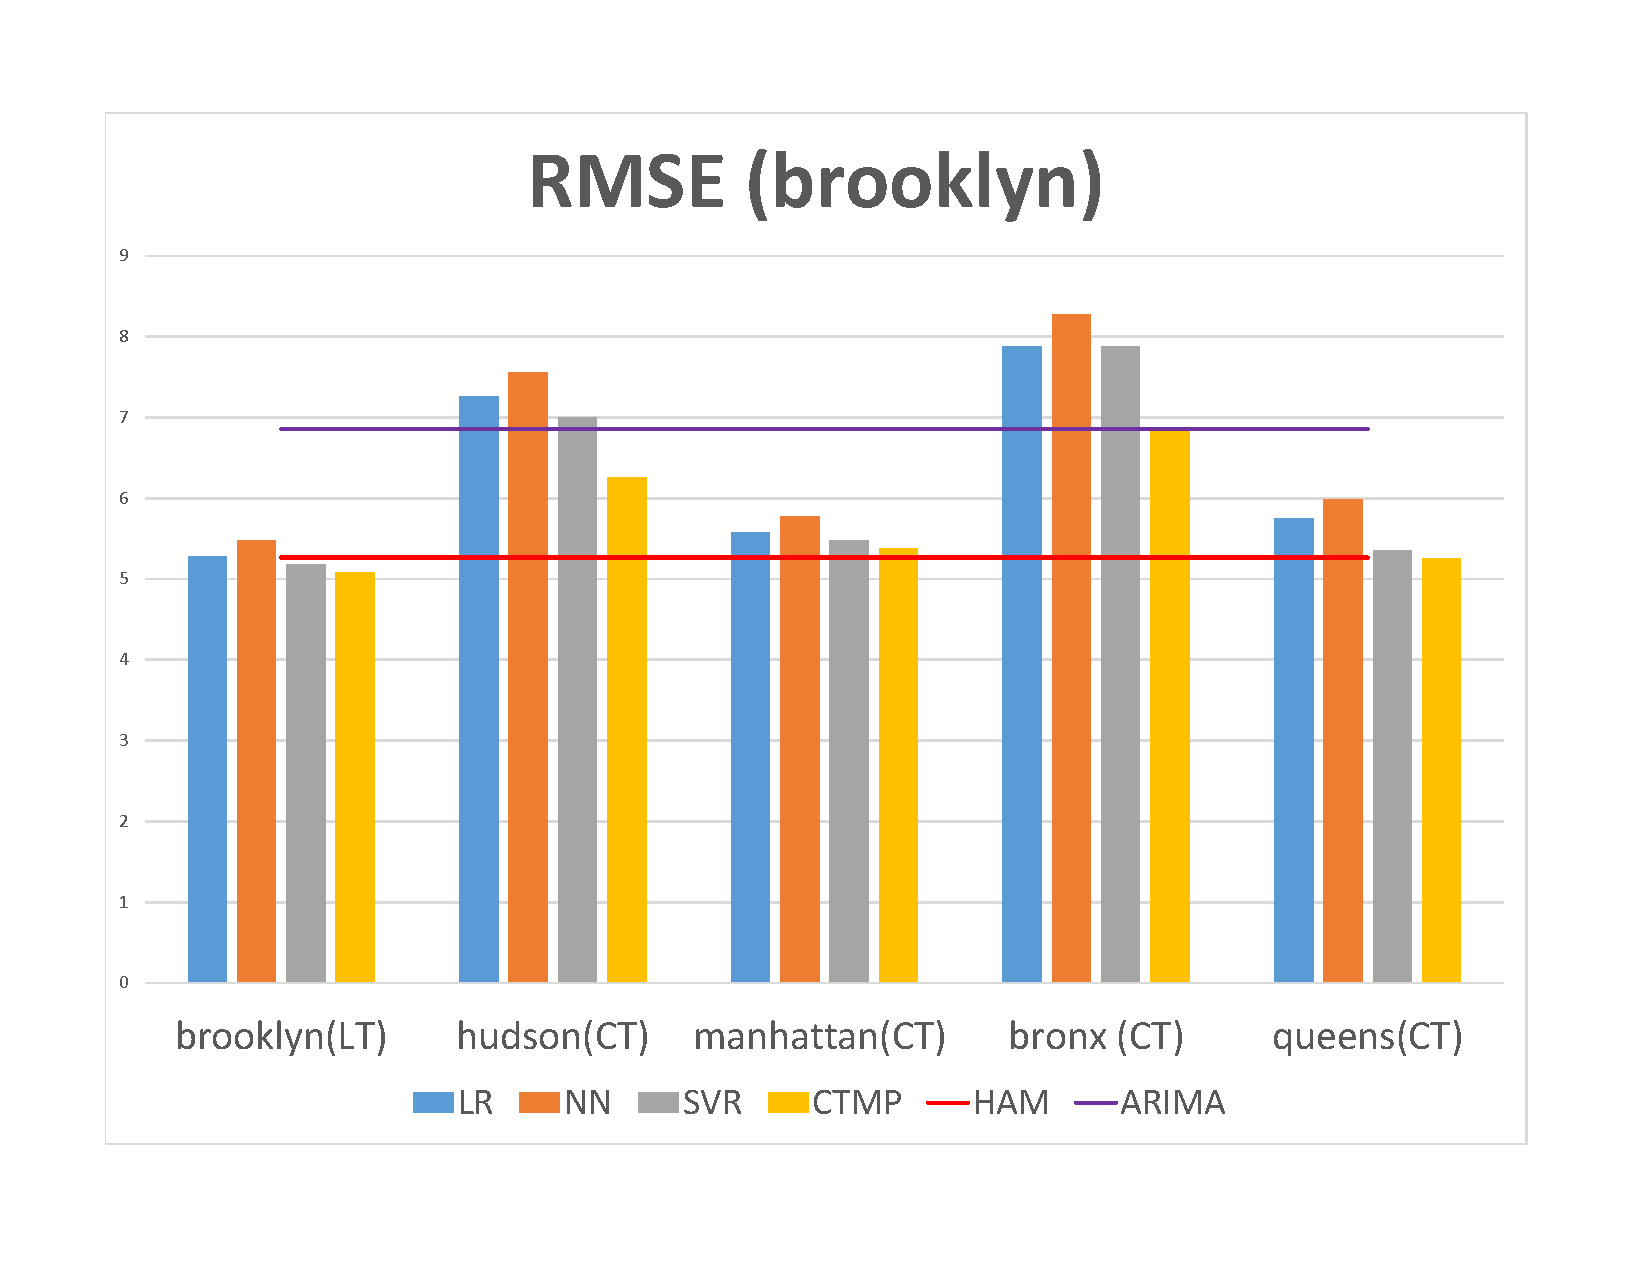
\includegraphics[width=0.32\textwidth]{figures/3.pdf}
	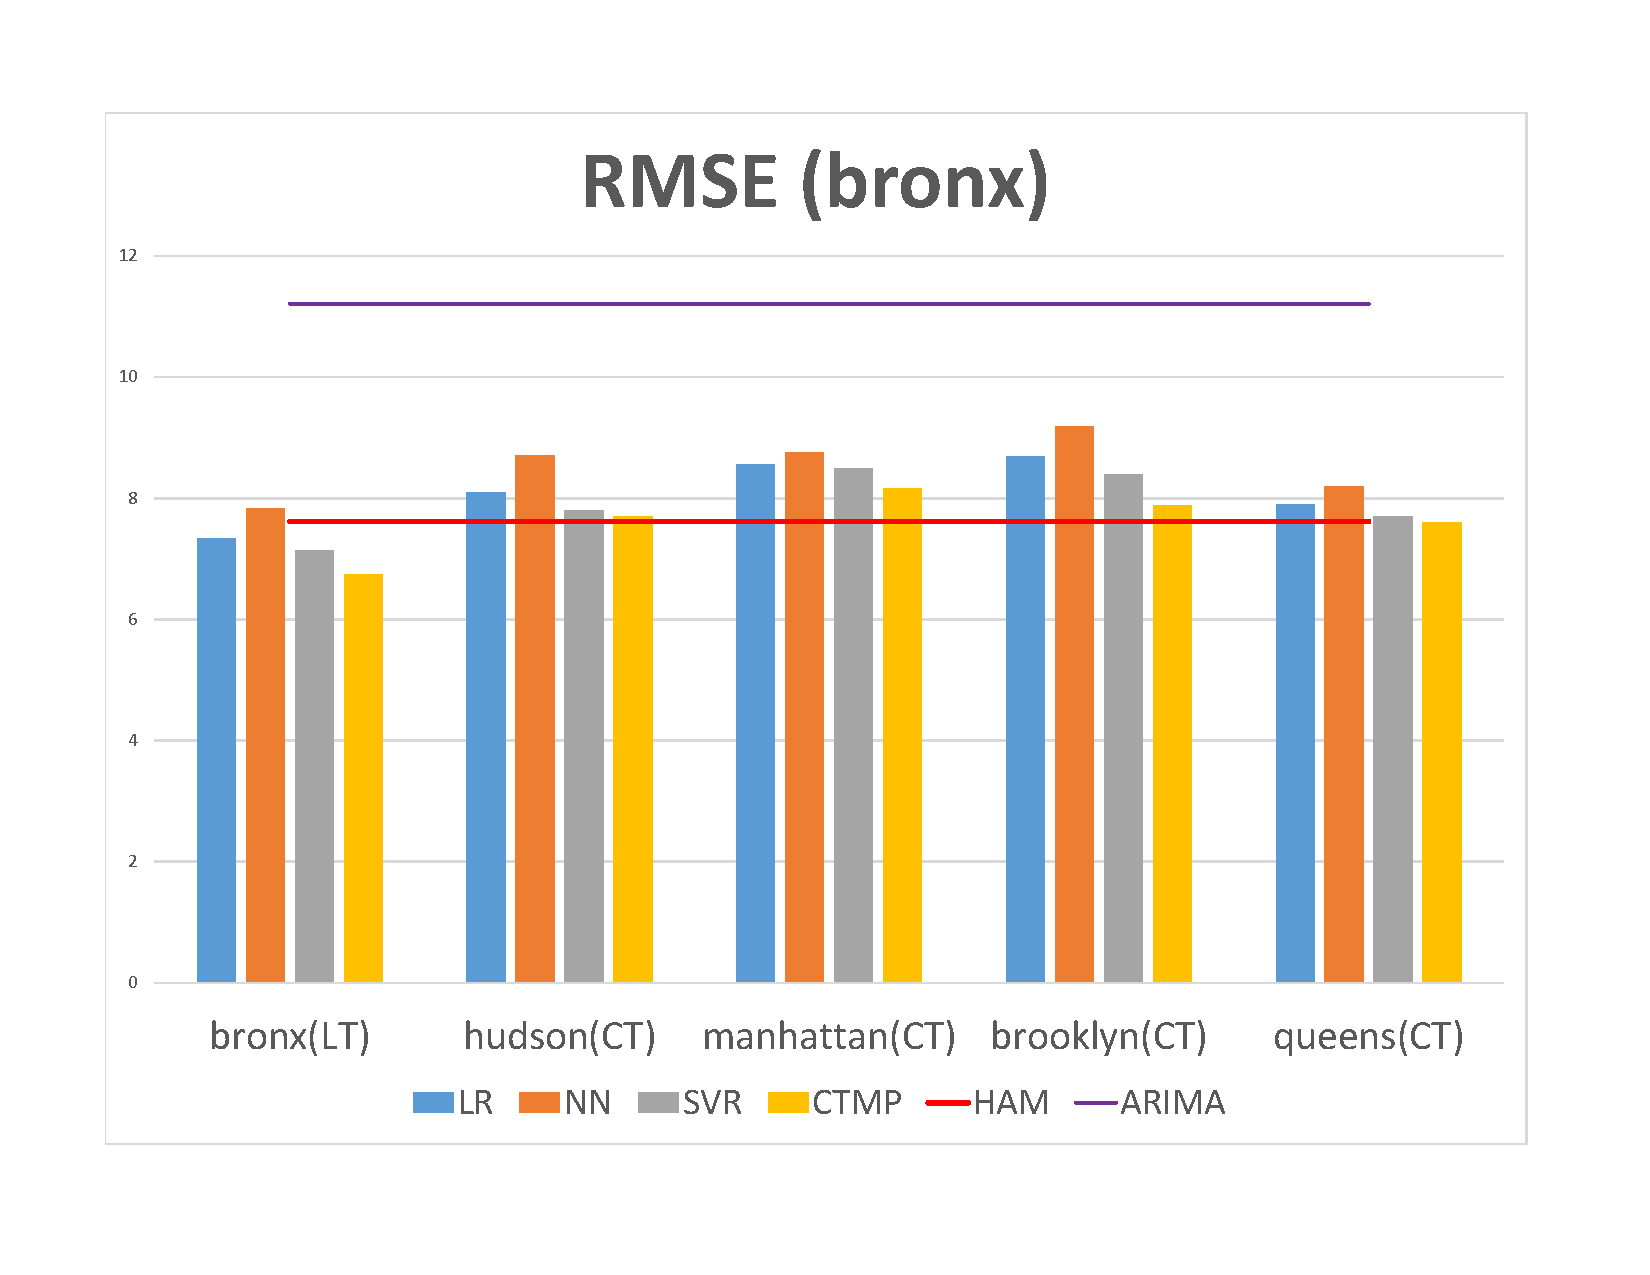
\includegraphics[width=0.32\textwidth]{figures/4.pdf}
	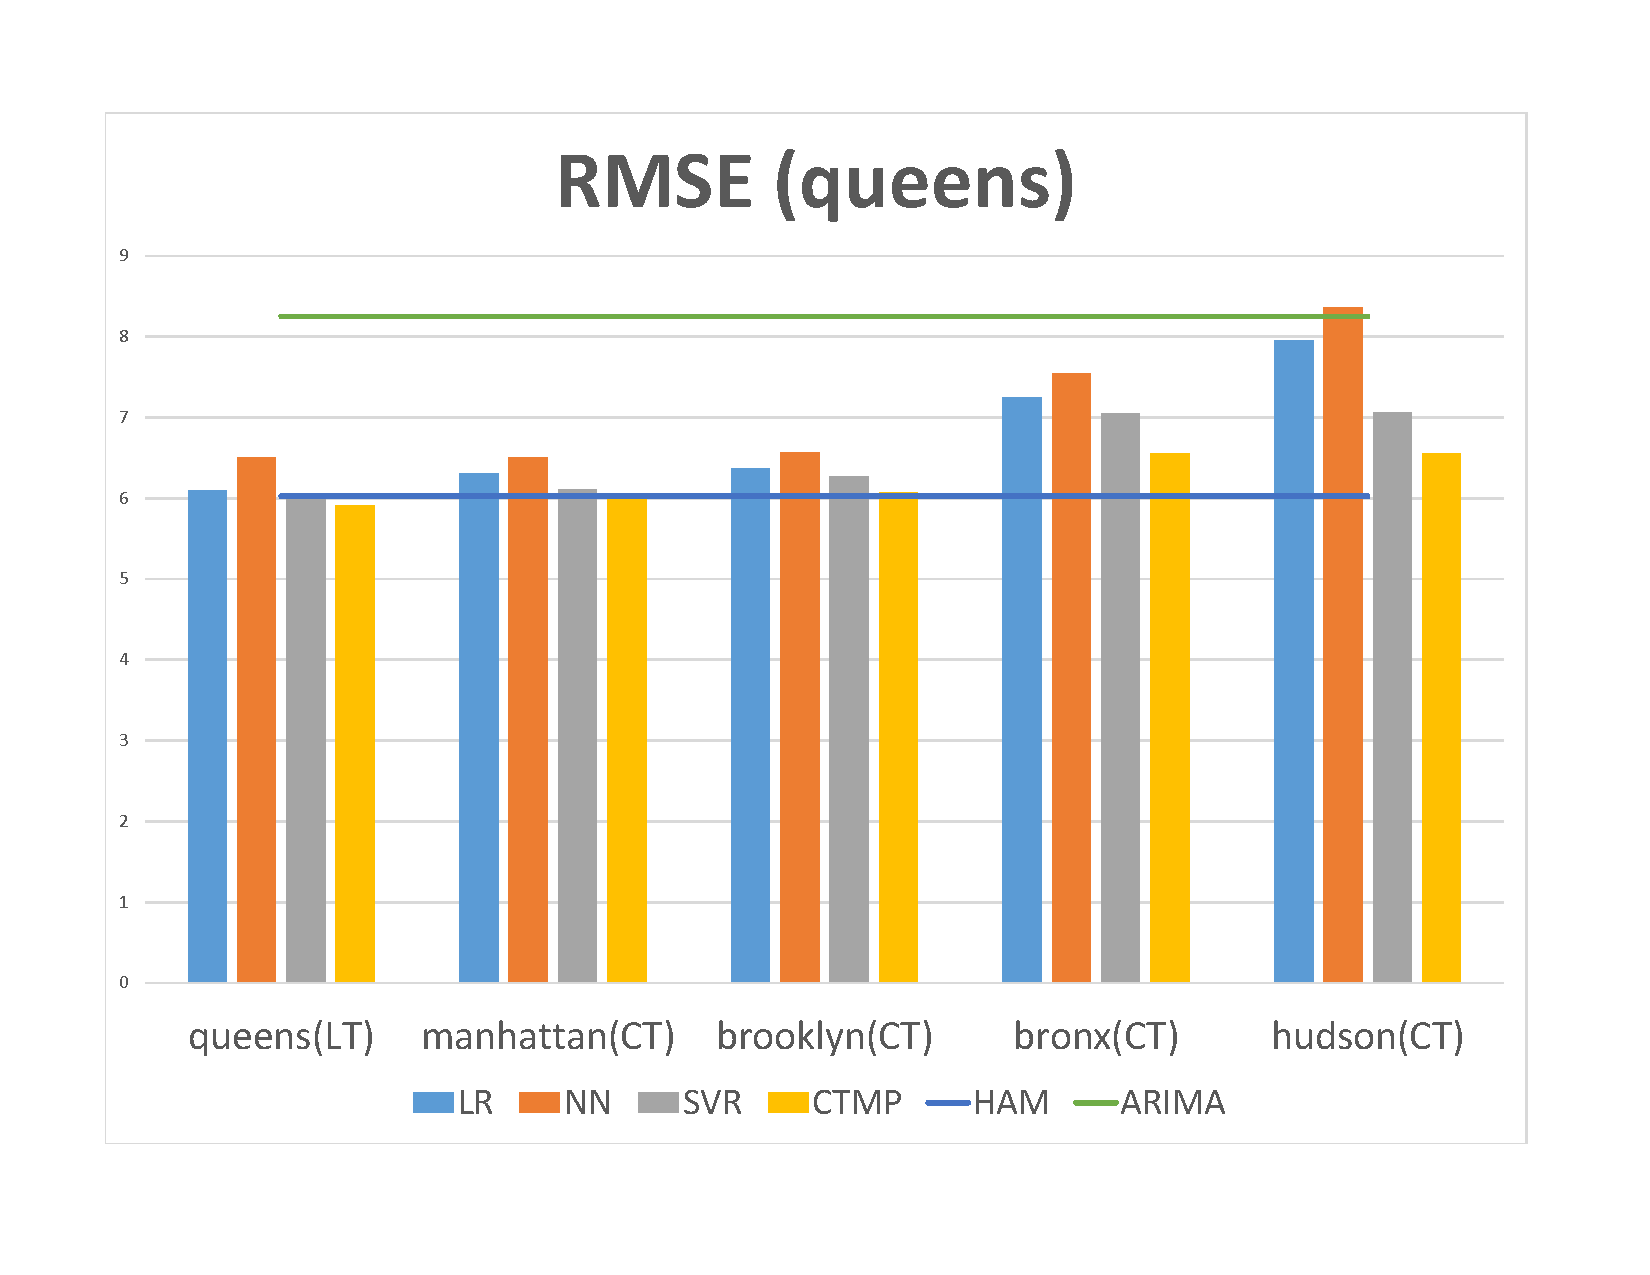
\includegraphics[width=0.32\textwidth]{figures/5.pdf}
	\caption{Local Transfer and Cross-region Transfer Performances in terms of RMSE; Each sub-figure is a about region, and each cluster is either a Local Transfer(LT) or a Cross-region Transfer(CT).}
	\label{fig:transfer}
\end{figure*}
Also, we present the results of both \textit{Local Transfer} (LT) and \textit{Cross-region Transfer} (CT) in Figure~\ref{fig:transfer}.
It can be concluded from each sub-figure that our methods achieve the similar RMSE with the HAM without explicitly using historical data for links in target areas.
Also, we can find that when the two regions are similar to each other, 
then when we cross-region transfer one to another the performance is still good. 
Sometimes, even our CT methods can achieve very similar results then HAM without using any historical data on the predicted areas, such as ``Manhattan'' $\rightarrow$ ``Queens'' in the last sub-figure.
Apart from that, we found that a larger region like ``Manhattan'' which contains various kinds of links will have better CT performance than other regions.
As for different prediction models, we found that our proposed CTPM performs better than other classic feature-based methods.
Whereas, NN model is relatively unstable. 



